

\chapter{R-package for model optimization (\software{mops})} \label{chap:mops}
\renewcommand{\tabdir}{chapters/mops/tab}
\renewcommand{\figdir}{chapters/mops/fig}

%%%%%%%%%%%%%%%%%%%%%%%%%%%%%%%%%%%%%%%%%%%%%%%%%%%%%%%%%%%%%%%%%%%%%%%%%%%%%%%%
%%%%%%%%%%%%%%%%%%%%%%%%%%%%%%%%%%%%%%%%%%%%%%%%%%%%%%%%%%%%%%%%%%%%%%%%%%%%%%%%
%%%%%%%%%%%%%%%%%%%%%%%%%%%%%%%%%%%%%%%%%%%%%%%%%%%%%%%%%%%%%%%%%%%%%%%%%%%%%%%%
\section{Purpose} \label{sec:mops:purpose}

The R-package \software{mops} provides a number of methods to facilitate the optimization of model parameters. The methods may be useful in the context of
\begin{itemize}
  \item model calibration.
  \item updating of operational models.
  \item optimization studies.
\end{itemize}

The methods provided in the \software{mops} package are designed for the following conditions:

\begin{itemize}
  \item The model, whose parameters are to be optimized, must be an executable file. In practice, this can be an executable built from source code (C++, FORTRAN, etc.) or a shell script. If it is a shell script, it typically calls an interpreter to process code written in a script language (R, Python, etc.).
  \item The executable must read the parameter values from plain text files. Thus, parameter values must \emph{not} be read from binary files or passed as command line arguments.
  \item The input parameters to be optimized must be floating point numbers. Internally, of course, the model can apply any kind of type conversion (typically to integer or logical).
  \item The text files holding the parameter values may be of arbitrary structure. However, the executable must read the numbers \emph{unformatted}. In other words, when reading a numeric value of one, for example, it must accept all of the following character representations \texttt{1}, \texttt{1.}, \texttt{1.0}, \texttt{1.0e+00}, \texttt{0.1e+01}. Note that legacy code sometimes uses \emph{formatted} read statements and may be incompatible with \software{mops}.
\end{itemize}

\software{echse}-based models generally comply with all of the conditions listed above.

%%%%%%%%%%%%%%%%%%%%%%%%%%%%%%%%%%%%%%%%%%%%%%%%%%%%%%%%%%%%%%%%%%%%%%%%%%%%%%%%
%%%%%%%%%%%%%%%%%%%%%%%%%%%%%%%%%%%%%%%%%%%%%%%%%%%%%%%%%%%%%%%%%%%%%%%%%%%%%%%%
%%%%%%%%%%%%%%%%%%%%%%%%%%%%%%%%%%%%%%%%%%%%%%%%%%%%%%%%%%%%%%%%%%%%%%%%%%%%%%%%
\section{Installation} \label{sec:mops:install}

The \software{mops} package is provided as a tarball. The package file name is \verb!mops_x.y.tar.gz! where x.y is a version number. See \citet{Echse-Install-Doc} for details on the installation procedure.

Note that the \software{mops} package depends on another R-package called \software{lhs} which allows for latin hypercube sampling. If the \software{lhs} package is not installed already, it needs to be downloaded and installed \emph{prior} to installing \software{mops}.

%%%%%%%%%%%%%%%%%%%%%%%%%%%%%%%%%%%%%%%%%%%%%%%%%%%%%%%%%%%%%%%%%%%%%%%%%%%%%%%%
%%%%%%%%%%%%%%%%%%%%%%%%%%%%%%%%%%%%%%%%%%%%%%%%%%%%%%%%%%%%%%%%%%%%%%%%%%%%%%%%
%%%%%%%%%%%%%%%%%%%%%%%%%%%%%%%%%%%%%%%%%%%%%%%%%%%%%%%%%%%%%%%%%%%%%%%%%%%%%%%%
\section{Standard documentation} \label{sec:mops:docs}

After the \software{mops} package has been loaded with the R command

\begin{lstlisting}[style=R]
library("mops")
\end{lstlisting}

a list of all provided methods can be generated with

\begin{lstlisting}[style=R]
help(package="mops")
\end{lstlisting}

The documentation of the individual methods can be displayed by typing the question mark followed by the name of the method, for example

\begin{lstlisting}[style=R]
?modelError_MCS
\end{lstlisting}

As always, the standard documentation for the methods is rather short. New users probably want to read the following sections to get a better understanding of the general concepts and the dependencies between the methods in the \software{mops} package.

%%%%%%%%%%%%%%%%%%%%%%%%%%%%%%%%%%%%%%%%%%%%%%%%%%%%%%%%%%%%%%%%%%%%%%%%%%%%%%%%
%%%%%%%%%%%%%%%%%%%%%%%%%%%%%%%%%%%%%%%%%%%%%%%%%%%%%%%%%%%%%%%%%%%%%%%%%%%%%%%%
%%%%%%%%%%%%%%%%%%%%%%%%%%%%%%%%%%%%%%%%%%%%%%%%%%%%%%%%%%%%%%%%%%%%%%%%%%%%%%%%
\section{Theoretical background} \label{sec:mops:background}

\subsection{Goal of optimization} \label{sec:mops:background:optimization:goal}

Optimization generally refers to the minimization\footnote{To solve a maximization problem, the objective function is simply multiplied by $-1$.} of the value of a function whose value depends on one or more parameters. This function is called the \emph{objective function}. Let's write the objective function as $f(p)$, with $f$ being the function's name and $p$ being a vector of parameters. In the special case of one-dimensional optimization, $p$ is simply a vector of length 1.

The goal of \emph{any} optimization procedure is to find a set of values for the parameters $p$ that minimizes the value of $f$.

\paragraph{Example 1 (minimization, 1-dimensional):} Determine the optimum dosage of a medicine for malaria protection that minimizes the total number of death from both infection and serious side effects ($f$: number of casualties, $p$: dosage).

\paragraph{Example 2 (maximization, 2-dimensional):} Determine the amounts of fertilizer and water to maximize the yield of a tomatoe field ($f$: yield, $p$: amounts of fertilizer and water).

\subsection{Optimization methods} \label{sec:mops:background:optimization:methods}

Depending on the nature of $f$ (non-linearities, discontinuities, local minima, etc.) and the number of unknown parameters in $p$, the optimization problem is more or less difficult to solve. Unfortunately, there is no general strategy that performs best in all cases. In fact, it is not even guaranteed that a $global$ minimum of $f$ is found at all.

One thing which is common to all optimization methods is that \emph{multiple} calls to $f$ for varying values of $p$ are necessary (bold arrow in \figref{fig:mops:concepts:optimization:multipleCalls_opt}). Only then, the effect of a change in the parameter value(s) $p$ on the value of $f$ can be detected.

\begin{figure}
  \centering
  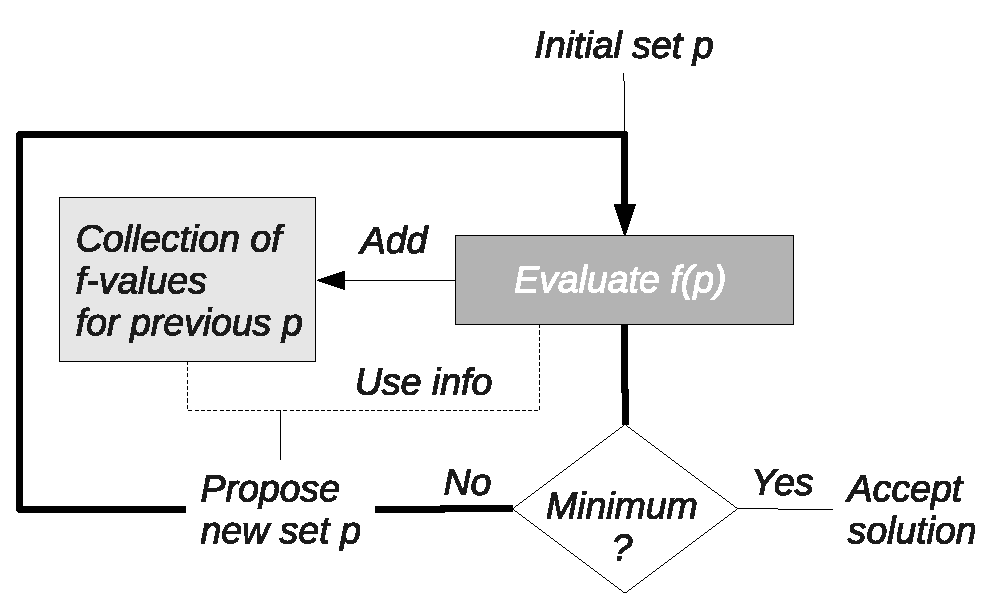
\includegraphics[width=0.9\columnwidth]{\figdir/multipleCalls_opt.eps}
  \caption{Basic outline of an optimization method. \label{fig:mops:concepts:optimization:multipleCalls_opt}}
\end{figure}

The basic strategies of optimization are distinguished by the way of how a new proposal for the values in $p$ is generated, given the information from the previous calls to $f$ for other values of $p$. The most important distinction is between \emph{deterministic} and \emph{stochastic} algorithms. Some examples and references for both types of strategies can be found in the help text of R's \texttt{optim} method.

As opposed to 'complete' optimization strategies, the technique of Monte-Carlo simulation does not identify a single optimum parameter set. Instead, the objective function is simply evaluated for a large number of random parameter sets (\figref{fig:mops:concepts:optimization:multipleCalls_mcs}). It is then up to a human to inspect the output and to draw conclusions on the suitability of parameter values.

\begin{figure}
  \centering
  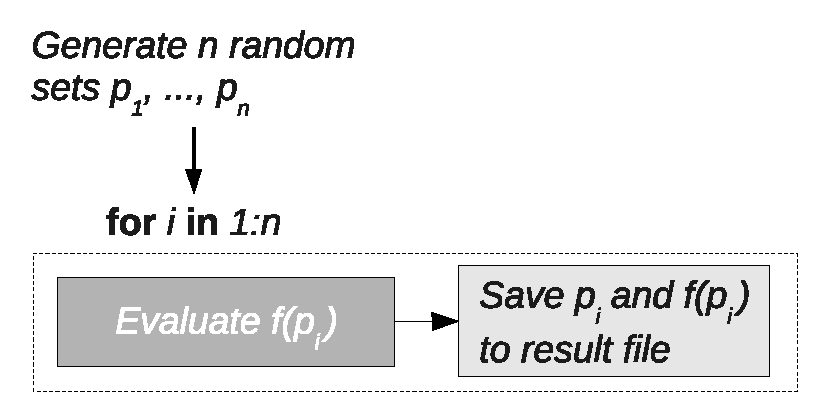
\includegraphics[width=0.7\columnwidth]{\figdir/multipleCalls_mcs.eps}
  \caption{Basic outline of Monte-Carlo simulation. \label{fig:mops:concepts:optimization:multipleCalls_mcs}}
\end{figure}

\subsection{Model error as objective function} \label{sec:mops:background:objFun}

In the context of a dynamic simulation, the objective function measures the deviation between a simulated time series (produced by the model) and a corresponding time series of observations. Generally, the deviation (synonyms: model error, performance, goodness-of-fit) depends on the values of the model's parameters. It may be helpful to see that this is very similar to the common case of fitting a linear model to a set of x,y-data (\figref{fig:mops:concepts:optimization:deviation}). The typical differences are:
\begin{itemize}
  \item In dynamic modeling, the x-axis represents the time.
  \item Real-world dynamic models often have more parameters than the linear model which has only 2 (slope and intercept).
  \item In many dynamic models, the relations between parameter values and the output are non-linear.
  \item In the case of dynamic simulation models, numerical methods are required to determine a set of optimum parameters (see \secref{sec:mops:background:optimization:methods}). For the linear model, an analytical expression exists to directly solve for slope and intercept.
\end{itemize}

\begin{figure}
  \centering
  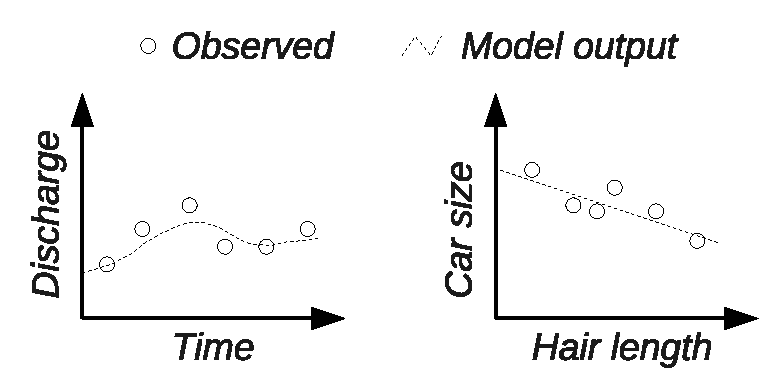
\includegraphics[width=0.9\columnwidth]{\figdir/deviation.eps}
  \caption{Goodness-of-fit for a dynamic simulation model (left) and an empirical linear model (right). \label{fig:mops:concepts:optimization:deviation}}
\end{figure}

The deviation between observations and the corresponding simulated values can be quantified by a variety of mathematical measures. In the case of linear fitting (\figref{fig:mops:concepts:optimization:deviation}, right), the sum of squared errors (SSE) is most often used. In dynamic modeling (\figref{fig:mops:concepts:optimization:deviation}, left), measures like the RMSE (root mean suared error) and the Nash-Sutcliffe index are usually preffered. They are based on the SSE as well but the values are more convenient to interpret.

In the context of dynamic modeling, the interior of a objective function $f(p)$ typically contains the steps listed in \tabref{tab:mops:background:objFun}.

\begin{table}
  \caption[Interior of an objective function in the context of dynamic modeling.]{Interior of an objective function in the context of dynamic modeling. It is assumed that the model reads all parameter values from text files. \label{tab:mops:background:objFun}}
  \begin{tabular}{p{0.03\columnwidth}p{0.85\columnwidth}} \hline\hline
  \# & Task \\ \hline
  1 & Get current parameter set $p$ (passed via the funcion's argument list). \\
  2 & Update the model's input files with the current values in $p$. \\
  3 & Run the model. \\
  4 & Read the model output (a time series). \\
  5 & Read observed data. \\
  6 & Compute the model error from the data read in steps 4 \& 5 using a suitable mathematical measure. \\
  7 & Return the result. \\ \hline\hline
  \end{tabular}
\end{table}

%%%%%%%%%%%%%%%%%%%%%%%%%%%%%%%%%%%%%%%%%%%%%%%%%%%%%%%%%%%%%%%%%%%%%%%%%%%%%%%%
\subsection{Semi-automatic calibration} \label{sec:mops:background:semiAutoCalib}

Environmental simulation models often have a large number of conceptual parameters whose values have to be calibrated based on observations. Without having a deeper understanding of the model's functioning, \ie{} the underlying equations, this is not a trivial task. Even if the equations are known, multi-dimensional, non-linear optimization remains a challenge and success is not guaranteed. The classic, deterministic optimization algorithms may fail for a number of reasons, such as truncation and round-off problems, insensitive parameters, complicated parameter interactions and compensations, non-continuous model behavior, or the existence of local minima. The alternative is the use of stochastic algorithms. Unfortunately, stochastic optimizers usually come with a number of algorithms parameters which affect convergence and computation times. If established general-purpose defaults do not exist, the estimation of these algorithm parameters is a problem on its own. Finally, a manual calibration by trial-and-error is often not practically feasible and the results have the reputation of being subjective.

Therefore, it is sometimes a good idea to fall back on the robust and straightforward concept of Monte-Carlo simulation (\figref{fig:mops:concepts:optimization:multipleCalls_mcs}). Some advantages of Monte-Carlo simulation are:
\begin{itemize}
  \item It simply cannot fail as long as the tested parameter sets do not cause invalid numeric results.
  \item There are no algorithm parameters.
  \item One can learn from the output about the (in)sensitivity of parameters, even if the model is a black box.
\end{itemize}

Especially useful is the concept of sequential Monte-Carlo simulation. This concept can be described by the following set of instructions:
\begin{description}
  \item[a)] Carry out a Monte-Carlo simulation with wide sampling ranges for all parameters.
  \item[b)] Visualize the results from step $a$. For each varied parameter, a scatter plot should be created with the parameter value on the x-axis and the model error on the y-axis.
  \item[c)] Inspect all plots created in step $b$. If a structure is visible in a plot, indicating an optimum range for the particular parameter, modify the sampling range of that parameter. Usually, the sampling range can be chosen narrower (unless the initial range was not wide enough).
  \item[d)] Return to step $a$, using the updated sampling range.
\end{description}

This semi-automatic approach to calibration has been successfully used in hydrological modeling \citep[see, \eg{}][]{Kneis2012}. It is certainly not among the most efficient strategies. However, the chance of complete failure is very low. Finally, with the above approach, it becomes visible whether the optimization problem is well behaved or of the nasty sort. Users of unsupervised optimization algorithms can only hope for a well behaved problem or guess on the cause of failure.

A practical example of parameter estimation using sequential Monte-Carlo simulation can be found in \secref{sec:mops:example_mcs:experiment}.

%%%%%%%%%%%%%%%%%%%%%%%%%%%%%%%%%%%%%%%%%%%%%%%%%%%%%%%%%%%%%%%%%%%%%%%%%%%%%%%%
%%%%%%%%%%%%%%%%%%%%%%%%%%%%%%%%%%%%%%%%%%%%%%%%%%%%%%%%%%%%%%%%%%%%%%%%%%%%%%%%
%%%%%%%%%%%%%%%%%%%%%%%%%%%%%%%%%%%%%%%%%%%%%%%%%%%%%%%%%%%%%%%%%%%%%%%%%%%%%%%%

\section{Important methods in \software{mops}} \label{sec:mops:methods}

\subsection{\function{update\_template}} \label{sec:mops:methods:update_template}

As illustrated in \figsref{fig:mops:concepts:optimization:multipleCalls_opt} and \ref{fig:mops:concepts:optimization:multipleCalls_mcs}, optimization methods and Monte-Carlo simulation involve many successive of evaluations of the objective functions for different parameter values. In each evaluation, the model's input files need to be updated (recall \tabref{tab:mops:background:objFun}). For this purpose, the \software{mops} package provides the \function{update\_template} method.

The method takes a template file and a \emph{named} vector of numerical values as input. It then scans the template file for the occurrence of \emph{placeholders}. A placeholder is a string enclosed by two designated characters, typically some sort of fancy brackets like \texttt{\{\}}, \texttt{[]} or \texttt{<>}. The \function{update\_template} method tries to replace every placeholder in the template file by the numerical value of a matching element from the input vector. A matching element is one whose name is identical to the placeholder's central string, \ie{} the string between the designated characters. The mode of action of the \function{update\_template} method is best demonstrated by the examples in \figsref{fig:mops:methods:update_template_example1} and \ref{fig:mops:methods:update_template_example2}.

\begin{figure}
  \centering
  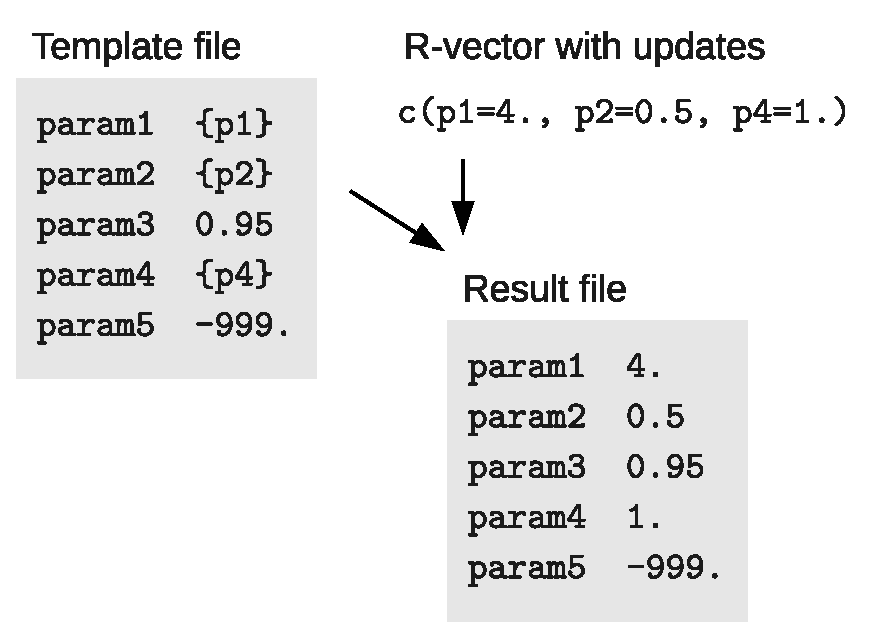
\includegraphics[width=0.7\columnwidth]{\figdir/update_template_example1.eps}
  \caption[Example application of the \texttt{update\_template} method.]{Example application of the \texttt{update\_template} method. Here, the characters to identify the start and the end of a placeholder are \texttt{``\{``} and \texttt{``\}``}, respectively. \label{fig:mops:methods:update_template_example1}}
\end{figure}

\begin{figure}
  \centering
  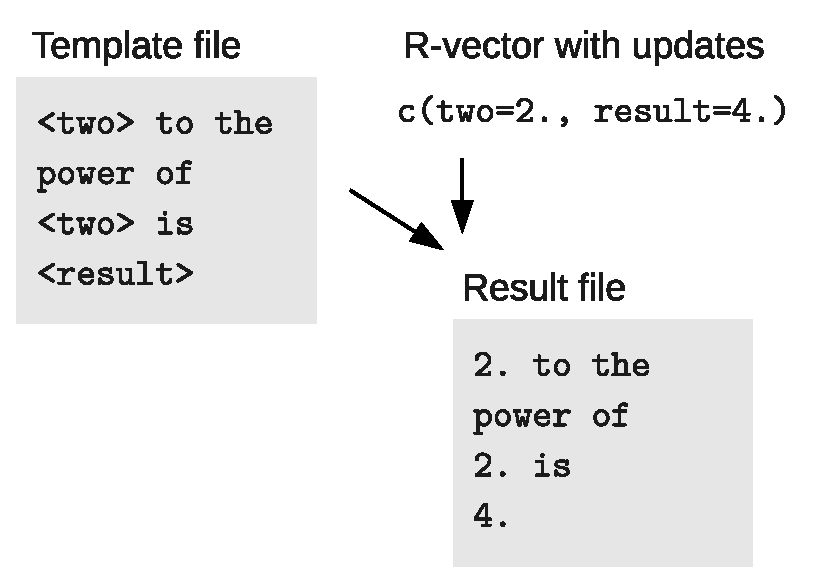
\includegraphics[width=0.7\columnwidth]{\figdir/update_template_example2.eps}
  \caption[Another example application of the \texttt{update\_template} method.]{Another example application of the \texttt{update\_template} method. Here, the characters to identify the start and the end of a placeholder are \texttt{``<``} and \texttt{``>``}, respectively. \label{fig:mops:methods:update_template_example2}}
\end{figure}

Although the \function{update\_template} can be called in isolation, it is mainly used as a sub-routine in other high-level methods of the \software{mops} package.

\subsection{\function{modelError\_multiDim}} \label{sec:mops:methods:modelError_multiDim}

The \function{modelError\_multiDim} is the central high-level method of the \software{mops} package. It represents a complete objective function. For a given parameter set, the method is able to perform all the steps listed in \tabref{tab:mops:background:objFun}. It can directly be used together with R's generic optimization method \texttt{optim}.

\subsection{\function{mcs\_run} and \function{mcs\_eval}} \label{sec:mops:methods:mcs}

The methods \function{mcs\_run} and \function{mcs\_eval} provide a complete framework for Monte-Carlo simulation. \function{mcs\_run} generates the random parameter sets and carries out all the simulations.  The function \function{mcs\_eval} calculates the corresponding model errors and creates graphics to summarize the results of Monte-Carlo experiments. A complete example for the use of these methods is provided in \secref{sec:mops:example_mcs}.

%%%%%%%%%%%%%%%%%%%%%%%%%%%%%%%%%%%%%%%%%%%%%%%%%%%%%%%%%%%%%%%%%%%%%%%%%%%%%%%%
%%%%%%%%%%%%%%%%%%%%%%%%%%%%%%%%%%%%%%%%%%%%%%%%%%%%%%%%%%%%%%%%%%%%%%%%%%%%%%%%
%%%%%%%%%%%%%%%%%%%%%%%%%%%%%%%%%%%%%%%%%%%%%%%%%%%%%%%%%%%%%%%%%%%%%%%%%%%%%%%%

\section{Example: Monte-Carlo simulation} \label{sec:mops:example_mcs}

%%%%%%%%%%%%%%%%%%%%%%%%%%%%%%%%%%%%%%%%%%%%%%%%%%%%%%%%%%%%%%%%%%%%%%%%%%%%%%%%
\subsection{Model equations} \label{sec:mops:example_mcs:modelEqn}

This section introduces the practical use of the \texttt{mcs\_run} method to perform a Monte-Carlo simulation. For the purpose of demonstration, we consider the fairly simple 1-dimensional advection-dispersion model (\eqnref{eqn:mops:example_mcs:modelEqn:ade-pde}). It describes the 1-dimensional (longitudinal) transport of dissolved, non-reactive matter in a river.

\begin{equation} \label{eqn:mops:example_mcs:modelEqn:ade-pde}
\dfrac{\partial c}{\partial t} = d \cdot \dfrac{\partial^2 c}{\partial x^2} - u \cdot \dfrac{\partial c}{\partial x}
\end{equation}

\begin{tabular}{lp{0.7\columnwidth}}
  $c$ & Concentration (g/m$^3$) \\
  $x$ & River station (m) \\
  $d$ & Dispersion coefficient in x-direction (m$^2$/s) \\
  $u$ & Average flow velocity in x-direction (m/s) \\
\end{tabular}

\medskip
This partial differential equation model has two parameters, $d$ and $u$. For certain conditions, \eqnref{eqn:mops:example_mcs:modelEqn:ade-pde} has the analytical solution presented in \eqnref{eqn:mops:example_mcs:modelEqn:ade-solution}.

\begin{equation} \label{eqn:mops:example_mcs:modelEqn:ade-solution}
  c(x,t)= \frac{m}{A \cdot \sqrt{4 \cdot \pi \cdot d \cdot t}} \cdot exp\left(\frac{-(x-u \cdot t)^2}{4 \cdot d \cdot t} \right)
\end{equation}

with the additional symbols

\begin{tabular}{lp{0.7\columnwidth}}
  $t$ & Time (s) \\
  $m$ & Mass (g) \\
  $A$ & Wet cross-section area (m$^2$) \\
\end{tabular}

\medskip
This solution assumes that
\begin{itemize}
  \item The injection of mass at $t=0$ occurs in an infinitesimally short time span.
  \item The mass is instantly distributed over the entire cross-section.
  \item The flow is steady (constant rate) and uniform (constant cross-section geometry).
\end{itemize}

The behavior of the model is illustrated in \figsref{fig:mops:example_mcs:modelEqn:fixedStations} and \ref{fig:mops:example_mcs:modelEqn:fixedTimes} for constant values of $m$=100, $a$=1, $d$=30, and $u$=0.5. \figref{fig:mops:example_mcs:modelEqn:fixedStations} shows the time series of concentration (chemographs) that one would obtain by frequent analysis of water samples taken at a particular river station. To get a picture as in \figref{fig:mops:example_mcs:modelEqn:fixedTimes}, one would have to organize synchronous sampling at multiple stations along the river.

\begin{figure}
  \centering
  \includegraphics[width=0.75\columnwidth]{\figdir/ad-equation_fixedStations.eps}
  \caption{Solutions of \eqnref{eqn:mops:example_mcs:modelEqn:ade-solution} at a fixed set of river stations for variable times. \label{fig:mops:example_mcs:modelEqn:fixedStations}}
\end{figure}

\begin{figure}
  \centering
  \includegraphics[width=0.75\columnwidth]{\figdir/ad-equation_fixedTimes.eps}
  \caption{Solutions of \eqnref{eqn:mops:example_mcs:modelEqn:ade-solution} at a fixed set of times for variable river stations. \label{fig:mops:example_mcs:modelEqn:fixedTimes}}
\end{figure}

%%%%%%%%%%%%%%%%%%%%%%%%%%%%%%%%%%%%%%%%%%%%%%%%%%%%%%%%%%%%%%%%%%%%%%%%%%%%%%%%
\subsection{Model implementation} \label{sec:mops:example_mcs:modelImpl}
The C++ source code listed in \figref{fig:mops:example_mcs:adModel_code} implements a simulation model based on the equations from \secref{sec:mops:example_mcs:modelEqn}. It solves \eqnref{eqn:mops:example_mcs:modelEqn:ade-solution} for a fixed station $x$ and an array of times. Thus, it computes a chemograph as in \figref{fig:mops:example_mcs:modelEqn:fixedStations}. For compatibility with the \software{mops} package, the executable reads all input data -- including the values of the two parameters $u$ and $d$ -- from a text file.

\begin{figure*}
  \lstinputlisting[style=c++]{\figdir/mcs_example/adModel.cpp}
  \caption{C++ source code of the advection-dispersion model (file: adModel.cpp). \label{fig:mops:example_mcs:adModel_code}}
\end{figure*}

To build an executable from the source code in \figref{fig:mops:example_mcs:adModel_code}, the GNU C++ compiler can be used \citep[see][for mode info]{Echse-Install-Doc}. Assuming that the source code is saved in a file 'adModel.cpp', an appropriate command line for compilation would be:

\begin{lstlisting}[style=shell]
  g++ -lstdc++ -o adModel adModel.cpp
\end{lstlisting}

The command should create an executable 'adModel' (possibly with an appropriate file name extension).

To successfully run the model, two command line arguments must be passed to the executable. The first argument is the name of the input file containing all input data, including the values of the parameters $u$ and $d$. The second command line argument is the name of the output file containing the simulated concentrations. An example of an appropriate input file is given in \figref{fig:mops:example_mcs:adModel_inputFixed}. The model expects to find the definition of a single input value per line. Each line should start with a string, representing the name of the input item, followed by one or more blank characters, followed by the value. The meaning of the values $u$, $d$, $a$, $m$, and $x$ is clear from \eqnsref{eqn:mops:example_mcs:modelEqn:ade-pde} and \ref{eqn:mops:example_mcs:modelEqn:ade-solution}. The two additional values define the array of times of interest. $tmax$ defines the upper limit of the simulation time (starting at zero) and $dt$ specifies the temporal resolution of the output. Both values are in units of seconds. The value of $dt$ should be less than $tmax$ to produce (any) useful output.

\begin{figure}
  \lstinputlisting[style=txt]{\figdir/mcs_example/in_fixedValues.txt}
  \caption{Sample input file for the model defined in \figref{fig:mops:example_mcs:adModel_code}. \label{fig:mops:example_mcs:adModel_inputFixed}}
\end{figure}

%%%%%%%%%%%%%%%%%%%%%%%%%%%%%%%%%%%%%%%%%%%%%%%%%%%%%%%%%%%%%%%%%%%%%%%%%%%%%%%%
\subsection{Observed data} \label{sec:mops:example_mcs:obsData}

\eqnref{eqn:mops:example_mcs:modelEqn:ade-solution} can be used to determine the average flow velocity $u$ and the longitudinal dispersion coefficient $d$ from tracer experiments. We assume that the set of observations given in \figref{fig:mops:example_mcs:adModel_observations} was obtained in such an experiment. In addition, we assume that
\begin{itemize}
  \item The observations were made at river station $x$= 1000 m while the injection took place at $x$=0.
  \item The river's wet cross-section area is $a$= 15 \sqm.
  \item The known input mass of the tracer was $m$= 5 g.
\end{itemize}

\begin{figure}
  \lstinputlisting[style=txt]{\figdir/mcs_example/observations.txt}
  \caption{Time series of observed concentrations (file: observations.txt). \label{fig:mops:example_mcs:adModel_observations}}
\end{figure}

%%%%%%%%%%%%%%%%%%%%%%%%%%%%%%%%%%%%%%%%%%%%%%%%%%%%%%%%%%%%%%%%%%%%%%%%%%%%%%%%
\subsection{Monte-Carlo experiment} \label{sec:mops:example_mcs:experiment}

\subsubsection*{Preparation of template file(s)}
The first step of setting up a Monte-Carlo simulation is the preparation of parameter template files. Since our model (\figref{fig:mops:example_mcs:adModel_code}) reads all data from a single file, we have to prepare a single template file only. To do so, we simply take the sample file from \figref{fig:mops:example_mcs:adModel_inputFixed} and substitute the values of the parameters of interest by appropriate placeholders. Using curly braces as the designated characters for placeholders, an appropriate template file could look as in \figref{fig:mops:example_mcs:adModel_inputTemplate}. In this example, the placeholders are named like the parameters. This is not a must but a simple and useful convention.

\begin{figure}
  \lstinputlisting[style=txt]{\figdir/mcs_example/in_template.txt}
  \caption{Template parameter file with placeholders for the values of the parameters $u$ and $d$ (cf. \figref{fig:mops:example_mcs:adModel_inputFixed}). \label{fig:mops:example_mcs:adModel_inputTemplate}}
\end{figure}

\subsubsection*{Writing a driver script in R}
The next step is to write an R script to call the \texttt{run\_mcs} method from the \software{mops} package with appropriate arguments. For our example, such a driver script is shown in \figref{fig:mops:example_mcs:driver}. The R script has been structured into several parts using comment lines. The subsequent paragraphs provide some details on the contents and meaning of these parts.

\paragraph{PART 0} This part accounts for initial actions. It clears R's memory of variables, loads the \software{mops} package, and sets the working directory. When using a copy of the code, the working directory needs to be adjusted to the local settings.

\paragraph{PART 1} In this part, the names of all files are defined which are created in part 3 of the script. This includes the model's input file (which is generated from a template) and the model's output file. It may be convenient to use temporary file and folder names.

\paragraph{PART 2} In this part, two tables are created (as \texttt{data.frame} objects). The first table defines the sampling ranges of the parameters and is passed as argument \texttt{ranges\_table} to the \function{mcs\_run} method in part 3. The second table holds information required for the automatic editing of the model's input files. It is passed as argument \texttt{updating\_table} to the \function{mcs\_run} method in part 3. In this example, the table consists of a single row because only a single file needs to be updated.

In the case of models with a larger number of parameters or multiple input files that need to be updated, is is better style to put the contents of the two table(s) in text file(s). Then, one can use R's \function{read.table} method to read the data and instantiate the \texttt{data.frame} objects.

\paragraph{PART 3} This part contains the call to the \texttt{run\_mcs} method. Information on all arguments can be found in the \software{mops} package's help files. Some additional hints related to the more complex arguments are given below:

\begin{itemize}
  \item In this example, it is assumed that the file name of the model executable is 'adModel' and that the file resides in the working directory (argument \texttt{model\_path}). The actual name depends on the output created by compiling the source code from \figref{fig:mops:example_mcs:adModel_code}.
  \item The model executable expects two \emph{unnamed} command line arguments (see code in \figref{fig:mops:example_mcs:adModel_code}). The two expected file names are supplied in an \emph{unnamed} vector to the argument \texttt{model\_args}.
  \item In this example, it is assumed that the observed data (\figref{fig:mops:example_mcs:adModel_observations}) reside in a file named 'observations.txt' (argument \texttt{obs\_file}). Furthermore, it is assumed that this is a TAB-separated file with the time in column 'time' and the observed values in column 'conc'.
  \item The functions assigned to the arguments \texttt{sim\_timeConv} and \texttt{obs\_timeConv} are identical. They convert a numical time into a value of R's \texttt{POSIXct} class. Here, the numerical time is the number of seconds after tracer injection (see \figref{fig:mops:example_mcs:adModel_observations} and the source code in \figref{fig:mops:example_mcs:adModel_code}). It does not matter which base time is used (here 1970-01-01 00:00:00) as long as it is identical for the observed and simulated time series.
  \item The value of the function assigned to argument \texttt{gof\_function} is returned as a \emph{named} vector. Using a named vector has the advantage that this name appears in the result file.
\end{itemize}

\paragraph{PART 4} This final part calls \function{mcs\_eval} to analyze and visualize the result of the Monte-Carlo experiment. For each parameter included in the experiment, a the marginal distribution of the model error is plotted in a separate sub-figure (see examples in \figsref{fig:mops:example_mcs:dottyplots_originalRange} and \ref{fig:mops:example_mcs:dottyplots_narrowedRange}). These plots are also known as 'dotty plots'.

\begin{figure*}
  \lstinputlisting[style=R]{\figdir/mcs_example/mcs_driver.r}
  \caption{R code to run the Monte-Carlo experiment using the \software{mops} package. \label{fig:mops:example_mcs:driver}}
\end{figure*}

\begin{figure}
  \centering
  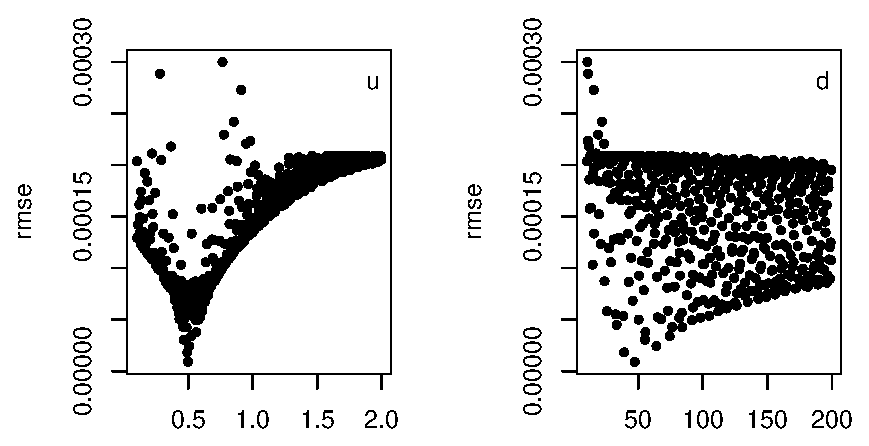
\includegraphics[width=0.9\columnwidth]{\figdir/mcs_example/dottyplots_originalRange.eps}
  \caption{Output graphics created by the R code from \figref{fig:mops:example_mcs:driver}. \label{fig:mops:example_mcs:dottyplots_originalRange}}
\end{figure}

\subsubsection*{Inspecting the output}

The graphical output from the R code (\figref{fig:mops:example_mcs:driver}) is presented in \figref{fig:mops:example_mcs:dottyplots_originalRange}. In this example with only two parameters ($u$ and $d$), some structure is visible in the plots of the marginal distributions. From the left sub-figure, one may conclude that a parameter value of $u \approx 0.5$ fits best with the observation data. The right sub-figure of \figref{fig:mops:example_mcs:dottyplots_originalRange} suggest that reasonable values for the dispersion coefficient $d$ are probably found in a range between 10 and 70. In order to refine the estimate, one could try different options:
\begin{enumerate}
  \item Re-run the Monte-Carlo experiment with narrower sampling ranges. For example, the sampling range for parameter $d$ could be restricted to 0 $\ldots$ 100. This option was already discussed in \secref{sec:mops:background:semiAutoCalib}. The result of such a re-run with narrowed sampling ranges is presented in \figref{fig:mops:example_mcs:dottyplots_narrowedRange}.
  \item Re-run the Monte-Carlo experiment with a higher number of random samples. 
  \item Use the current estimates of $u=0.5$ and $d=50$ as initial values for one of the true optimization algorithms provided by R's \texttt{optim} method.
\end{enumerate}

\begin{figure}
  \centering
  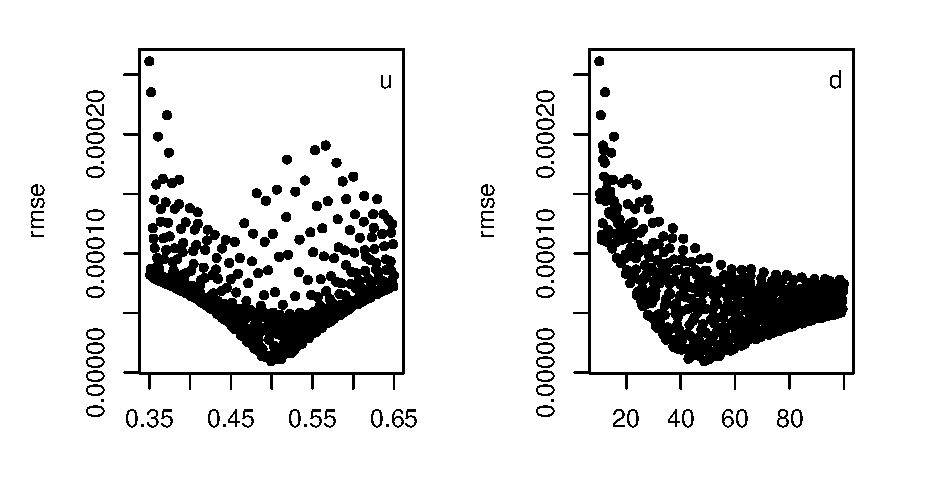
\includegraphics[width=0.9\columnwidth]{\figdir/mcs_example/dottyplots_narrowedRange.eps}
  \caption{Output graphics created by the R code from \figref{fig:mops:example_mcs:driver} after narrowing of the sampling ranges ($u$ in 0.35 $\ldots$ 0.65; $d$ in 10 $ \ldots$ 100). \label{fig:mops:example_mcs:dottyplots_narrowedRange}}
\end{figure}

%%%%%%%%%%%%%%%%%%%%%%%%%%%%%%%%%%%%%%%%%%%%%%%%%%%%%%%%%%%%%%%%%%%%%%%%%%%%%%%%
\section{Using \software{mops} with an \software{echse}-based model} \label{sec:mops:echse}

This section contains some practical hints for the use of \software{mops} together with an \software{echse}-based model. The hints refer in particular to the methods \texttt{modelError\_multiDim} and \texttt{modelError\_oneDim} which have many arguments in common.

\paragraph{Command line arguments} An \software{echse}-based model generally expects some mandatory command line arguments of the form 'key=value' \citep[see][for details]{Echse-Main-Doc}. All optional command line arguments (configuration data) are of the 'key=value' form as well. Therefore, the value assigned to the method's argument \texttt{model\_args} must always be a \emph{named} vector. A minimum exaple, covering only the mandatory command line arguments is given in \figref{fig:mops:echse:cmdArgs}.

\begin{figure}
\begin{lstlisting}[style=R]
model_args= c(file_control="myModel.cnf",
  file_log="myModel.log",
  file_err="errors.html",
  format_err="html", silent="true")
\end{lstlisting}
\caption{Example, demonstrating the use of the \texttt{model\_args} argument. \label{fig:mops:echse:cmdArgs}}
\end{figure}

\paragraph{Clean-up functions} An \software{echse}-based model never overwrites existing files. Therefore, when carrying out a series of model runs, there must be a mechanism to delete the output created by the previous run. By assigning a proper function to the arguments \texttt{func\_first} and an appropriate value to \texttt{moreArgs\_first} such an automatic clean-up may be accomplished. Alternatively, the clean-up may be done right after a model run, by supplying an appropriate function for \texttt{func\_final} and value for \texttt{moreArgs\_final}.

In some cases, a complete removal of the model outputs after each run may be undesired. For example, one might be interested in the actual time series output produced by the individual runs of a Monte-Carlo simulation. Then, renaming is usually an appropriate alternative to deletion of files. This can be done, for example, by supplying appropriate code as \texttt{func\_final} and a suitable value for \texttt{moreArgs\_final}. In those cases, it is often convenient to use a string representation of the system's time for the generation of unique file names.

\paragraph{Files created by the model} Output files created by an \software{echse}-based model conform to some simple standards which facilitates the use of \software{mops}. In all time series output files, the column with time information is named 'end\_of\_interval'. Thus, this is the string to be assigned to the argument \texttt{sim\_colTime} (\figref{fig:mops:echse:time}). Furthermore, the time information printed by \software{echse}-based models is always in ISO 8601 format (YYYY-MM-DD hh:mm:ss) with date and time separated by a single blank character. This is also the default format used by \software{mops}. Therefore, the actual argument for \texttt{sim\_timeConv} can be omitted in the call to methods like \texttt{modelError\_MCS}. If, even though, a time-conversion function is specified it should be defined as in \figref{fig:mops:echse:time}.

\begin{figure}
\begin{lstlisting}[style=R]
  sim_colTime=  "end_of_interval"
  sim_timeConv= function(x) {
    as.POSIXct(strptime(x,
    "%Y-%m-%d %H:%M:%S",tz="GMT"),
    tz="GMT")
    }
\end{lstlisting}
\caption{Appropriate values of the arguments \texttt{sim\_colTime} and \texttt{sim\_timeConv} when using \software{mops}'s methods with an \software{echse}-based model. \label{fig:mops:echse:time}}
\end{figure}

%%%%%%%%%%%%%%%%%%%%%%%%%%%%%%%%%%%%%%%%%%%%%%%%%%%%%%%%%%%%%%%%%%%%%%%%%%%%%%%%
\section{Troubleshooting} \label{sec:mops:troubleshooting}

\subsection{General recommendations} \label{sec:mops:troubleshooting:general}

The methods contained in the \software{mops} package perform quite complex tasks and there is a high potential for making mistakes. In many cases, the cause of failure should be obvious from the generated error messages. However, there are situations where it may be difficult to locate and identify the actual problem. Therefore, some general guidelines for troubleshooting are given in this section. More specific problems are addressed in \secref{sec:mops:troubleshooting:specific}.

If one of \software{mops}'s high-level methods involving a call to a simulation model fails, one should first try to find out at which step of the computation the problem occurred. There are four possible categories a--d with typical symptoms:

\subsubsection*{(a) Stop occurs prior to running the model}
\begin{itemize}
  \item The model does neither produce the desired output nor any other files (log files, files with error messages, etc.).
  \item A return code of the model is \emph{not} reported.
\end{itemize}

\subsubsection*{(b) Stop occurs when calling the model}
\begin{itemize}
 \item As in case (a), the model does not produce any output files.
  \item A \emph{non-zero} return code of the model \emph{is} reported.
\end{itemize}

\subsubsection*{(c) Stop occurs while running the model}
\begin{itemize}
  \item The model produces a file with error messages and/or a log file whose entries indicate early termination.
  \item A \emph{non-zero} return code of the model \emph{is} reported.
\end{itemize}

\subsubsection*{(d) Stop occurs after running the model}
\begin{itemize}
  \item The model produces the desired output files and possibly a complete log file.
  \item A return code of the model is \emph{not} reported.
\end{itemize}

Note that (b) is a quite common case. It typically occurs if the model is called with invalid or incomplete command line arguments. In case of \software{echse}-based models, it may happen that the model executable is called successfully but the names of the files for log info and diagnostic messages are not properly passed via the command line. Consequently, the model terminates without creating any log or error output. The non-zero return level is the only sign of failure then.

\subsection{Specific recommendations} \label{sec:mops:troubleshooting:specific}

\subsubsection*{The model does not run at all}
\begin{itemize}
  \item Check the path to the executable if a relative or absolute path was specified.
  \item If the executable is called just by its name but the file does not reside in R's working directory, you might need to check/adjust your 'PATH' environment variable.
  \item Check for broken links (if a link is used).
  \item Check whether the file is actually executable.
\end{itemize}

\subsubsection*{The command line is not passed to the model}
\begin{itemize}
  \item Try to call the executable directly, \ie{} not via an intermediate shell script and not using a link. This is best done by adding the directory containing the executable to the 'PATH' variable.
  \item If this does not help, replace the executable by a shell script that reports its full command line but does nothing else. Try to learn from this.
\end{itemize}

\subsubsection*{The model crashes due to floating point exceptions}

In true optimization as well as in Monte-Carlo simulation, the simulation model is run with many different parameter sets. In general, the tested parameter sets are chosen by the used algorithm, based on sophisticated rules or simply by random sampling. Thus, the particular sets are not know a-priori.

In many models, the values of different parameters are not totally independent. For example, if a fictive parameter 'maximumCapacity' has a value of 5, it does not make sense if a companion parameter 'minimumCapacity' has a value greater than 5. Similarly, some parameter values may be incompatible with the initial value(s) of state variable(s). If, for example, the fictive parameter 'minTemperature' has a value of 5, problems are waiting to happen if a related state variable 'temperature' is initialized to a value of 0.

The consequences are as follows:
\begin{itemize}
  \item When using one of \software{mops}'s methods together with a true optimization algorithm, it may be necessary to set box-constraints for critical parameters. Similarly, when doing Monte-Carlo simulations with the \texttt{modelError\_MCS} method, the sampling ranges must be chosen with care in order not to produce invalid (\eg{} unphysical) parameter combinations.
  \item The initial values for the state variables must be chosen so as to be compatible with any parameter sets possibly tested during optimization or Monte-Carlo simulation, respectively.
\end{itemize}

Disregard of this often causes a model to crash due to floating point exceptions. In other cases, the model only produces implausible outputs (which are hopefully detected because of a bad fit).


